\section{Energy Production}
While the uptake of nutrients provides essential resources, some of which are
utilized to build the lipid scaffold housing the transporters, the variety of
metabolic pathways must then consume and generate energy in the form of NTPs
to build new cell mass. The high-energy phosophodiester bonds of (primarily)
ATP power a variety of cellular processes that drive biological systems away
from thermodynamic equilibrium. The next set of processes we consider as a
potential bottleneck in growth is the synthesis of ATP from ADP and inorganic
phosphate as well as maintenance of the electrochemical proton gradient which
powers it.

\subsection{ATP Synthesis}
Hydrolysis of the terminal phosphodiester bond of ATP into ADP (or
alternatively GTP and GDP) and an inorganic phosphate provides the kinetic driving
force in a wide array of biochemical reactions. One such reaction is the
formation of peptide bonds during translation, which requires $\approx$ 2 ATPs
for the charging of an amino acid to the tRNA and $\approx$ 2 GTP for the
formation of each peptide bond. Assuming the ATP costs
associated with error correction and post-translational modifications of
proteins are negligible, we can make the approximation that each peptide bond
has a net cost of $\approx$ 4 ATP (BNID: 101442, \cite{milo2010}). Formation
of GTP from ATP is achieved via the action of nucleoside diphosphate kinase,
which catalyzes this reaction without an energy investment \citep{lascu2000}
and therefore consider all NTP requirements of the cell to be functionally
equivalent to being exclusively ATP. In total, the energetic costs of peptide
bond formation consume $\approx$ 80\% of the cells ATP budget (BNID: 107782;
106158; 101637; 111918, \cite{lynch2015,stouthamer1973}). The pool of ATP is
produced by the F$_1$-F$_0$ ATP synthase -- a membrane-bound rotary motor
which under ideal conditions can yield $\approx$ 300 ATP per second (BNID:
114701; \cite{weber2003}).

To estimate the total number of ATP equivalents consumed during a cell cycle,
we will make the approximation that there are $\approx 3\times10^6$ proteins
per cell with an average protein length of $\approx$ 300 peptide bonds (BNID:
115702; 108986; 104877). Taking these values together, we find that the
typical \textit{E. coli} cell consumes $\sim 5 \times 10^9$ ATP per cell
cycle on protein synthesis alone. Assuming that each ATP synthases operates at
its maximal speed (300 ATP per second per synthase), $\approx$ 3000 ATP synthases are
needed to keep up with the energy demands of the cell. This estimate and a
is comparable with the experimental observations,  shown in \FIG{energy_production} (A). Much as we did for the estimates of transporter copy
numbers, we can generalize this estimate across different growth rates (indicated by the gray
line in \FIG{energy_production}), which appears to capture the growth rate
dependence of ATP synthase abundance. We note that this estimate assumes all ATP
is synthesized via ATP synthase and neglects synthesis via fermentative
metabolism. This assumption may explain why at the fastest growth rates
($\approx$ 2 hr$^{-1}$), our continuum estimate predicts more synthase than is
experimentally observed. Recent work has shown that at rapid growth rates,
\textit{E. coli} enters a stage of overflow metabolism where fermentative metabolism
becomes pronounced \cite{szenk2017}. 


\subsection{Generating the Proton Electrochemical Gradient}
In order to produce ATP, the F$_1$-F$_0$ ATP synthase itself must consume
energy. Rather than burning through its own product (and violating
thermodynamics), this intricate macromolecular machine has evolved to exploit
the electrochemical potential established across the inner membrane through
cellular respiration. This electrochemical gradient is manifest by the pumping
of protons into the intermembrane space via the electron transport chains as
they reduce NADH. In \textit{E. coli}, this potential difference is $\approx
-$200 mV (BNID: 102120). A simple estimate of the inner membrane as a capacitor
with a working voltage of -200 mV reveals that $\approx 2\times 10^4$ protons
must be present in the intermembrane space. However, the constant rotation of the ATP synthases would abolish
this potential difference in a few milliseconds if it were not being actively
maintained. 

% . To
% undergo a complete rotation (and produce a single ATP), the F$_1$-F$_0$ ATP
% synthase must shuttle $\approx$ 4 protons across the membrane into the
% cytosol (BNID: 103390). With $\approx$ 3000 ATP synthases each
% generating 300 ATP per second, the $2 \times 10^4$ protons establishing the 200
% mV potential would be consumed in only a few milliseconds. This brings us
% to our next estimate: how many electron transport complexes are needed to
% support the consumption rate of the ATP synthases?

The electrochemistry of the electron transport complexes of \textit{E. coli}
have been the subject of intense biochemical and biophysical study
\citep{ingledew1984, khademian2017,cox1970,henkel2014}. A recent work
\citep{szenk2017} examined the respiratory capacity of the \textit{E. coli}
electron transport complexes using structural and biochemical data, revealing
that each electron transport chain rapidly pumps protons into the
intermembrane space at a rate of $\approx$ 1500 protons per second (BIND:
114704; 114687). Using our estimate of the number of ATP synthases required
per cell [\FIG{energy_production}(A)], coupled with these recent
measurements, we estimate that $\approx 1000$ electron transport complexes
would be necessary to facilitate the $\sim 5 \times 10^6$ protons per second
diet of the cellular ATP synthases. This estimate is in agreement with the
number of complexes identified in the proteomic datasets (plot in
\FIG{energy_production}(B)). This suggests that every ATP synthase must be
accompanied by $\approx$ 1 functional electron transport chain. Again, to
consider whether energy production may become a rate-limiting step in growth,
we need to consider whether cells could simply increase their abundances in
the cell membrane, and we turn our attention towards the available space in
the membrane next.

% Again, if
% this were a rate limiting process for bacterial growth, one must conclude
% that it is not possible for the cell to simply increase the production of
% both the number of electron transport chain complexes as well as ATP
% synthases. As both of these components only function while bound to the inner
% membrane, we now turn our attention towards the available space in the
% membrane as well as surface-area-to-volume constraints.


\begin{figure}
    \begin{fullwidth}
        \centering{
            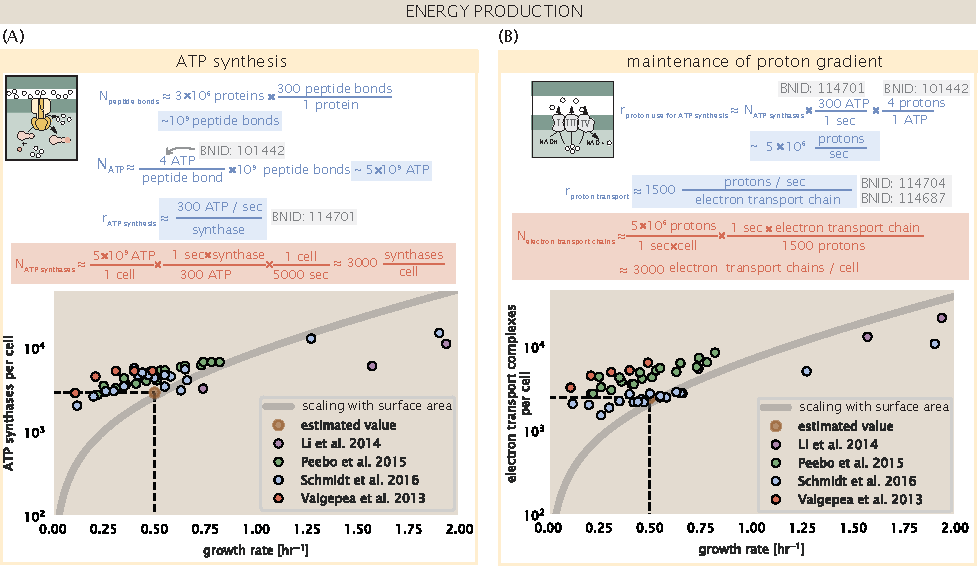
\includegraphics{main_figs/fig4_energy_production.pdf}
            \caption{\textbf{The abundance of F$_1$-F$_0$ ATP synthases and
            electron transport chain complexes as a function of growth
            rate.} (A) Estimate of the number of F$_1$-F$_0$ ATP synthase
            complexes needed to accommodate peptide bond formation and other NTP
            dependent processes. Points in plot correspond to the
            mean number of complete F$_1$-F$_0$ ATP synthase complexes that
            can be formed given proteomic measurements and the subunit
            stoichiometry
            [AtpE]$_{10}$[AtpF]$_2$[AtpB][AtpC][AtpH][AtpA]$_{3}$[AtpG][AtpD]$_3$.
            (B) Estimate of the number of electron transport chain complexes
            needed to maintain a membrane potential of $-$200 mV given
            estimate of number of F$_1$-F$_0$ ATP synthases from (A). Points
            in plot correspond to the average number of complexes identified
            as being involved in aerobic respiration by the Gene Ontology
            identifier GO:0019646 that could be formed given proteomic
            observations. These complexes include cytochromes \textit{bd1}
            ([CydA][CydB][CydX][CydH]), \textit{bdII} ([AppC][AppB]),
            \textit{bo$_3$},([CyoD][CyoA][CyoB][CyoC]) and NADH:quinone
            oxioreducase I
            ([NuoA][NuoH][NuoJ][NuoK][NuoL][NuoM][NuoN][NuoB][NuoC][NuoE][NuoF][NuoG][NuoI])
            and II ([Ndh]). Grey lines in both (A) and (B) correspond to the
            estimate procedure described, but applied to a continuum of growth
            rates. We direct the reader to the Supporting Information for a more
            thorough description of this approach.}
        \label{fig:energy_production}
        }
    \end{fullwidth}
\end{figure}


\section{Biosynthesis in a Crowded Membrane}
Our estimates thus far have focused on biochemistry at the periphery of the
cell and have generally been concordant with the abundances expected from simple
estimates. Furthermore, we have been able to describe the growth-rate dependeces
considering increasing cell volume and/or surface area. However, as surface area
and cell volume do not scale identically, it is worth considering what physical
limits may be imposed for transport or energy production given the ratio of
surface area to volume (S/V), which decreases with increasing growth rate.

% considered so far is performed Recall however that each transport process, as well as the ATP production via
% respiration, is performed at the bacterial membrane.
% This means that their
% maximum productivity can only increase in proportion to the cell's surface
% area divided by the cell doubling time.

% This difference in scaling would vary
% in proportion to the surface area-to-volume (S/V) ratio. Earlier we found
% that there was more than sufficient membrane real estate for carbon intake in
% our earlier estimate. However, since the total number of ATP synthases and
% electron chain transport complexes both exhibit a clear increase in copy
% number with growth rate, it was important to also consider the consequences
% of this S/V ratio scaling in more detail.

In our estimate of ATP production above we found that a cell demands about $5
\times 10^9$ ATP per cell cycle or $10^6$ ATP/s. With a cell volume of roughly 1
fL (BNID: 100004), this corresponds to about $2 \times 10^{10}$ ATP per fL of cell volume, in
line with previous estimates \citep{stouthamer1977, szenk2017}. In
\FIG{energy_scaling} (A) we plot this ATP demand as a function of the S/V ratio
in green, where we have considered a range of cell shapes from spherical to
rod-shaped with an aspect ratio (length/width) equal to 4. In order to consider
the maximum ATP that could be produced, we consider the amount of ATP that can
be generated by a membrane filled with ATP synthase and electron transport
complexes, which provides a maximal production of about 3 ATP / (nm$^2 \cdot$s)
\citep{szenk2017}. This is shown in blue in \FIG{energy_scaling}(A), which shows
that at least for the growth rates observed (right column in plot), the energy
demand is roughly an order of magnitude less. Interestingly, \cite{szenk2017}
also found that ATP production by respiration is less efficient than by
fermentation per membrane area occupied due to the additional proteins of the
electron transport chain. This suggests that, even under anaerobic growth, there
will be sufficient membrane space for ATP production.

The analysis highlights the diminishing capacity to provide resources as the
cell increases in size. However, the maximum energy production in
\FIG{energy_scaling}(A) does represents a somewhat unachievable limit since
the inner membrane must also include other proteins including those required
for lipid and membrane synthesis. To better
understand the overall proteomic makeup of the inner membrane, we therefore
used Gene Ontology (GO) annotations \citep{ashburner2000,
thegeneOntologyconsortium2018} to identify all proteins embedded or
peripheral to the inner membrane (GO term: 0005886). Those associated but not
membrane-bound include proteins like MreB and FtsZ%$, that traverse the inner %kmembrane by treadmilling %
and must nonetheless be considered as a vital
component occupying space on the membrane. In \FIG{energy_scaling}(B), we
find that the total protein mass per \textmu m$^2$ is nearly constant across
growth rates. Interestingly, when we consider the distribution of proteins
grouped by their Clusters of Orthologous Groups (COG) \citep{tatusov2000},
the relative abundance for those in metabolism (including ATP synthesis via
respiration) is also relatively constant across growth rates, suggesting that
no one process (energy production, nutrient uptake, etc.) is particularly
dominating even at fast growth rates \FIG{energy_scaling}(C).

\begin{figure}
    \begin{fullwidth}
        \centering{
            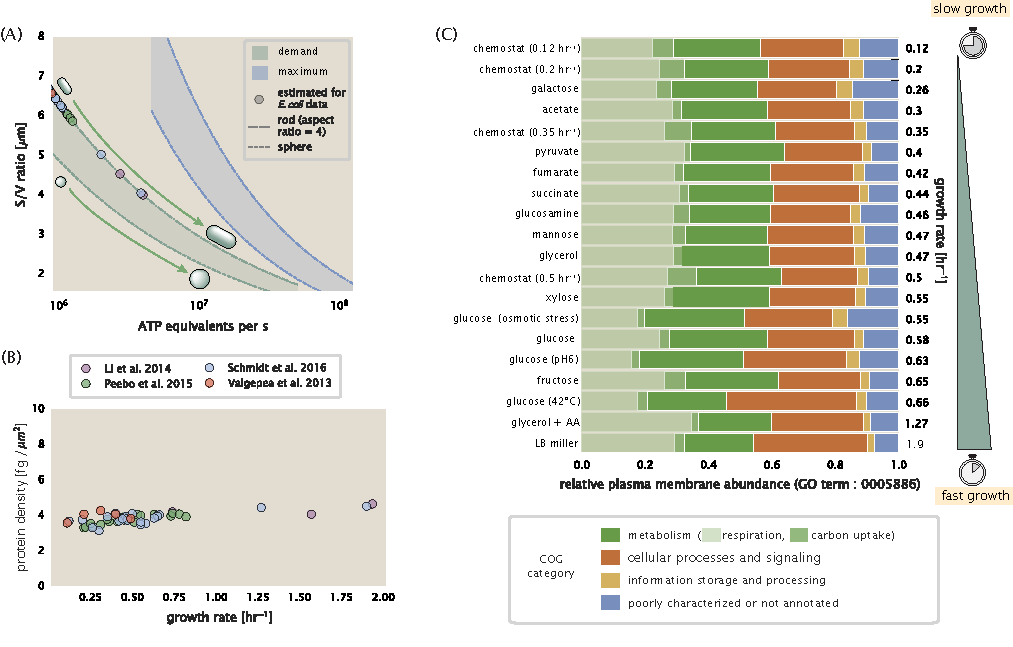
\includegraphics{main_figs/fig5_energy_SV_scaling.pdf}
            \caption{\textbf{Influence of cell size and S/V ratio on ATP
            production and inner membrane composition.} (A) Scaling of ATP
            demand and maximum ATP production as a function of S/V ratio.
            Cell volumes of 0.5 fL to 50 fL were considered, with the dashed
            (\texttt{- -}) line corresponding to a sphere and the dash-dot
            line (\texttt{-.}) reflecting a rod-shaped bacterium like
            \textit{E. coli} with a typical aspect ratio (length / width) of
            4 \citep{shi2018}. Approximately 50\% of the bacterial inner
            membrane is assumed to be protein, with the remainder lipid. The
            right plot shows the measured growth rates, and their estimated
            S/V ratio using growth rate dependent size measurements from
            \cite{si2017} (See Appendix \nameref{sec:protein_size_SV} on
            calculation). (B) Total protein mass per \textmu m$^2$ calculated
            for proteins with inner membrane annotation (GO term: 0005886).
            (C) Relative protein abundances by mass based on COG annotation.
            Metabolic proteins are further separated into respiration
            (F$_1$-F$_0$ ATP synthase, NADH dehydrogenase I,
            succinate:quinone oxidoreductase, cytochrome bo$_3$ ubiquinol
            oxidase, cytochrome bd-I ubiquinol oxidase) and carbohydrate
            transport (GO term: GO:0008643). Note that the elongation factor
            EF-Tu can also associate with the inner membrane, but was
            excluded in this analysis due to its high relative abundance
            (roughly identical to the summed protein shown in part
            (B)).}\label{fig:energy_scaling}
            }
                \end{fullwidth}
\end{figure}
